% Created 2023-02-09 Thu 17:46
% Intended LaTeX compiler: lualatex
\documentclass[11pt]{article}
\usepackage{graphicx}
\usepackage{longtable}
\usepackage{wrapfig}
\usepackage{rotating}
\usepackage[normalem]{ulem}
\usepackage{amsmath}
\usepackage{amssymb}
\usepackage{capt-of}
\usepackage{hyperref}
\usepackage{minted}
\usepackage{physics}
\usepackage[margin=0.5in]{geometry}
\author{David Lewis}
\date{\today}
\title{Lecture 9}
\hypersetup{
 pdfauthor={David Lewis},
 pdftitle={Lecture 9},
 pdfkeywords={},
 pdfsubject={},
 pdfcreator={Emacs 28.2 (Org mode 9.6)}, 
 pdflang={English}}
\begin{document}

\maketitle
\section*{1.}
\label{sec:org49a0587}
\begin{center}
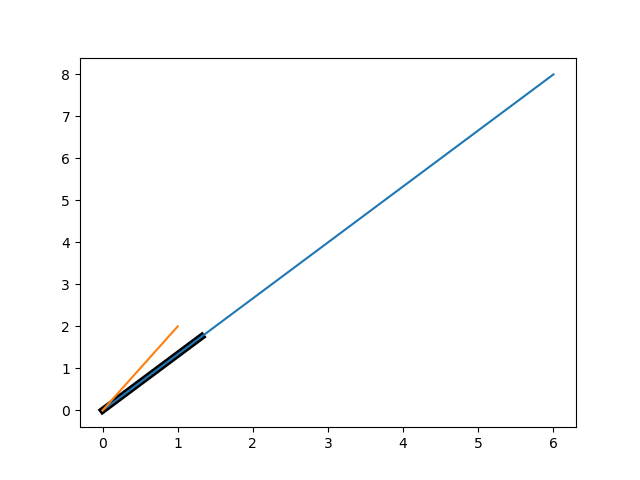
\includegraphics[width=0.8 \textwidth]{1.pdf}
\end{center}
\section*{2.}
\label{sec:org18f612b}
\begin{center}
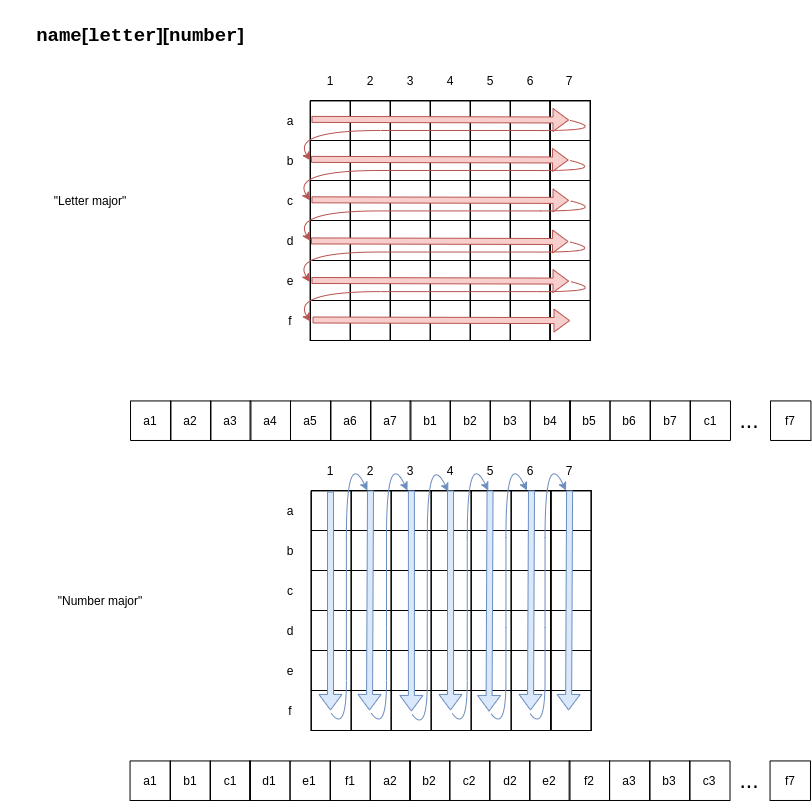
\includegraphics[width=0.8 \textwidth]{2.pdf}
\end{center}
\section*{3.}
\label{sec:org0e7e1b2}
\subsection*{a.}
\label{sec:org9f6e0d5}
\begin{center}
\begin{tabular}{rrrr}
A & B & C & D\\
\hline
1 & 1 & 4 & 4\\
2 & 2 & 5 & 5\\
3 & 3 & 6 & 6\\
4 & 4 & 7 & 7\\
5 & 5 & 8 & 8\\
\end{tabular}
\end{center}
\subsection*{b, c, d, e, f.}
\label{sec:orgf9d1add}
\begin{center}
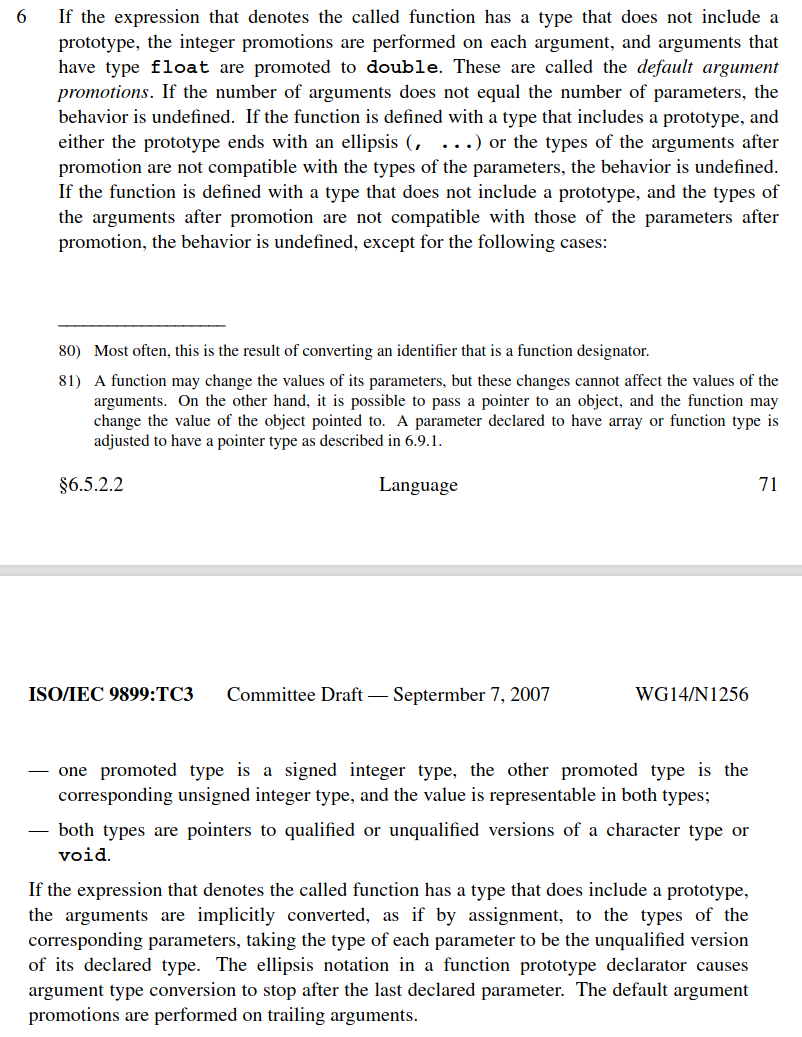
\includegraphics[width=0.8 \textwidth]{3.pdf}
\end{center}
\subsection*{g.}
\label{sec:orgb6d7d43}
It is possible, but not necessary if the objective is to find the itemsets with
minimum support. In the algorithm, all the possiblilites have already been
expanded, so there is no need to do so again.
\section*{4.}
\label{sec:org684851b}
\subsection*{a.}
\label{sec:org40f7111}
\begin{center}
\includegraphics[width=0.8 \textwidth]{4a.pdf}
\end{center}

\subsection*{b.}
\label{sec:org77cee51}
The order is in increasing order of support. This makes sense because it is an
inversion of how the tree is created. Projecting the tree removes the least
common item in the set, making the remaining tree more likely to occur.

\subsection*{c.}
\label{sec:org5df37a1}
\begin{center}
\includegraphics[width=0.8 \textwidth]{4b.pdf}
\end{center}
\end{document}
